\documentclass{beamer}
\usepackage{verbatim}
\usepackage{wrapfig}
\usepackage{color}
%\usetheme{Warsaw}
\usetheme[pageofpages=of,% String used between the current page and the
                         % total page count.
          bullet=circle,% Use circles instead of squares for bullets.
          titleline=true,% Show a line below the frame title.
          %titlepagelogo=opensuse,
          alternativetitlepage=true,% Use the fancy title page.
          ]{Torino}

\title{Enlightening Lizards}
\subtitle{Getting the Enlightenment experience \& Being a part of the effort}
\author{\texorpdfstring{Alex-P. Natsios\newline\url{drakevr@2f30.org}}{Author}}
%\author{Alex-P. Natsios}
\institute{Fosscomm 2015 - Athens}
\date{7 Nov 2015}
\begin{document}
    \begin{frame}
       \titlepage
    \end{frame}

    \begin{frame}{\$ whoami}
        \begin{itemize}
            \item Alexandros-Panayiotis Natsios
            \item IRC Handle: Drakevr
            \item cs undergrad student @ teilar.gr
            \item openSUSE Advocate
            \item Enlightenment Enthusiast and Contributor
        \end{itemize}
    \end{frame}

    \begin{frame}
        \center\huge A bit of history\ldots
    \end{frame}

    \begin{frame}{Enlightenment? What in the \ldots}

        {\bf Enlightenment}, also known simply as {\bf E}, was initially
        developed before even 1996 but the current iteration of the window
        manager (the Environment as we know it today) started with the version
        {\bf 0.17.0} which was in development for {\bf 12} years.
        {\bf Enlightenment 17} as it was called wasn't packaged in {\bf openSUSE}
        until a little after it's stable release in 21 December 2012

    \end{frame}

    \begin{frame}{A Slightly different environment \ldots}{Desktop Environment vs. Desktop Shell}
        \begin{block}{Desktop Environment}
            It is an implementation of the Desktop metaphor, made of a bundle of
            applications running on top of the base Operating System(OS). which
            share a common Graphical User Interface (GUI), a common look and
            feel and are working together to bring a complete experience to the
            user.
        \end{block}

        \begin{block}{Window Manager}
            A window manager is system software that controls the placement and
            appearance of windows.
            It usually works in conjunction with a Desktop Environment (and is
            thus designed around one).
        \end{block}
    \end{frame}

    \begin{frame}{A Slightly different environment \ldots}{cont.}
        \begin{block}{Desktop Shell}
            A Desktop Shell is something inbetween the two. \\
            It provides more than {\bf just} a window manager but not enough to
            be considered a full fledged Desktop Environment.
        \end{block}
    \end{frame}

    \begin{frame}
        \center\huge A Quick Glance
    \end{frame}

    \begin{frame}{A View to a desktop}
        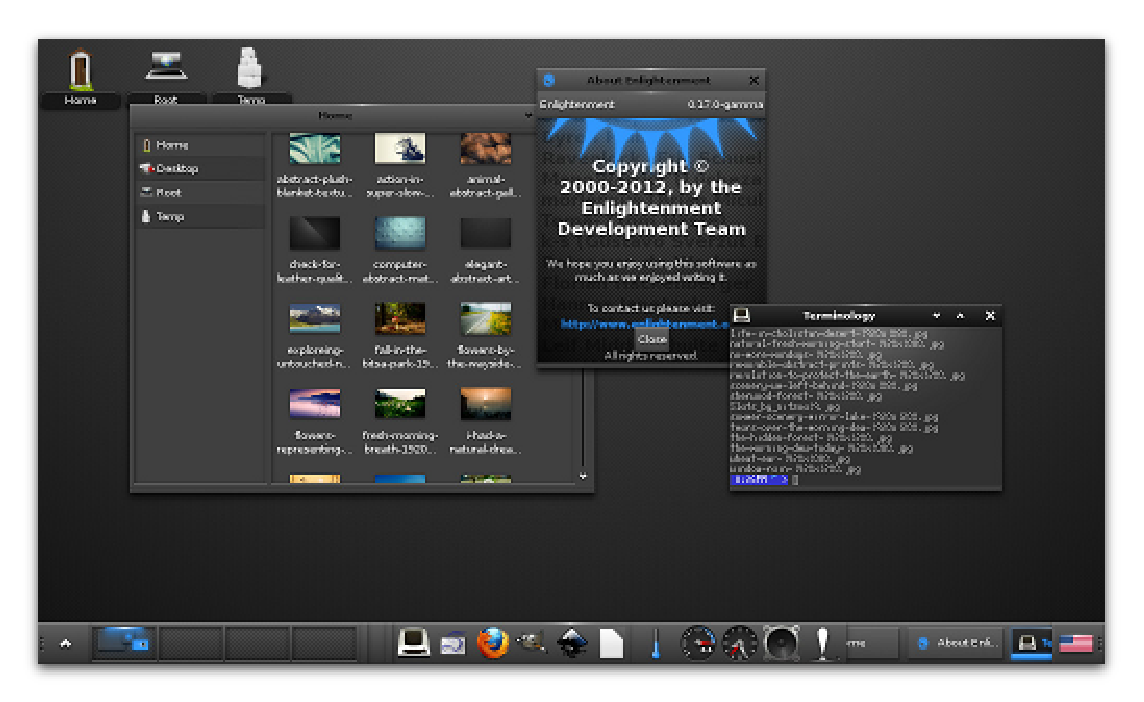
\includegraphics[scale=0.5]{img/e-shot-main.eps}
    \end{frame}

    \begin{frame}{Desktop Royale}
        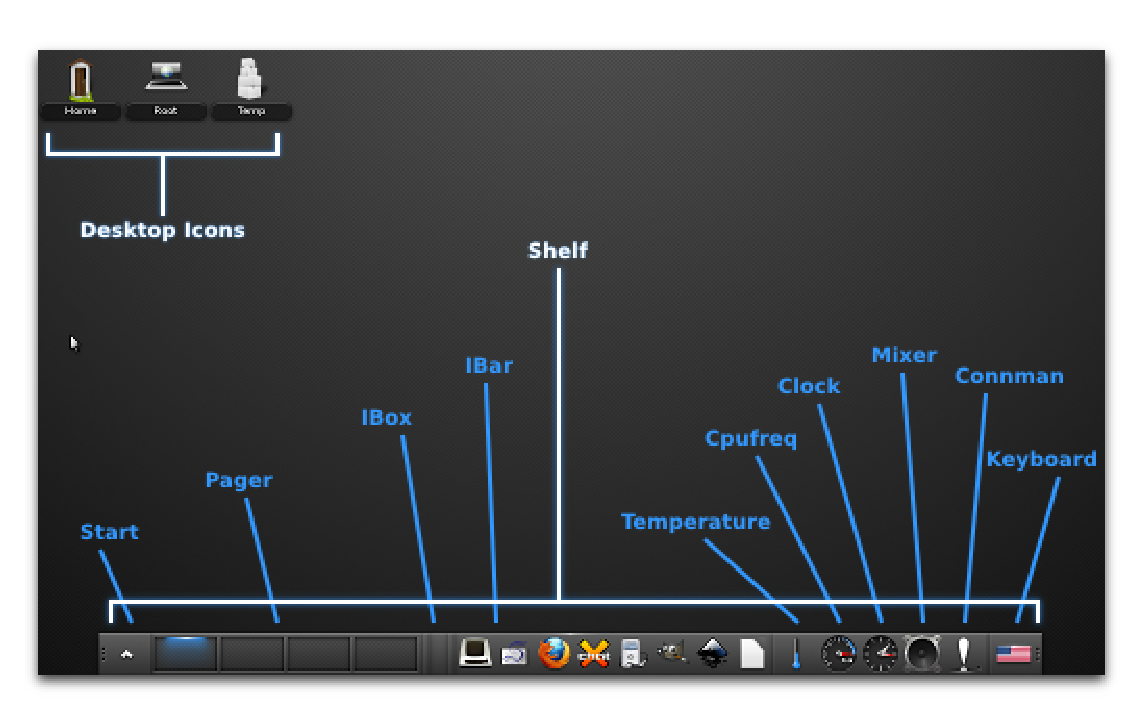
\includegraphics[scale=0.5]{img/e-elements.eps}
    \end{frame}

    \begin{frame}{License to start}
        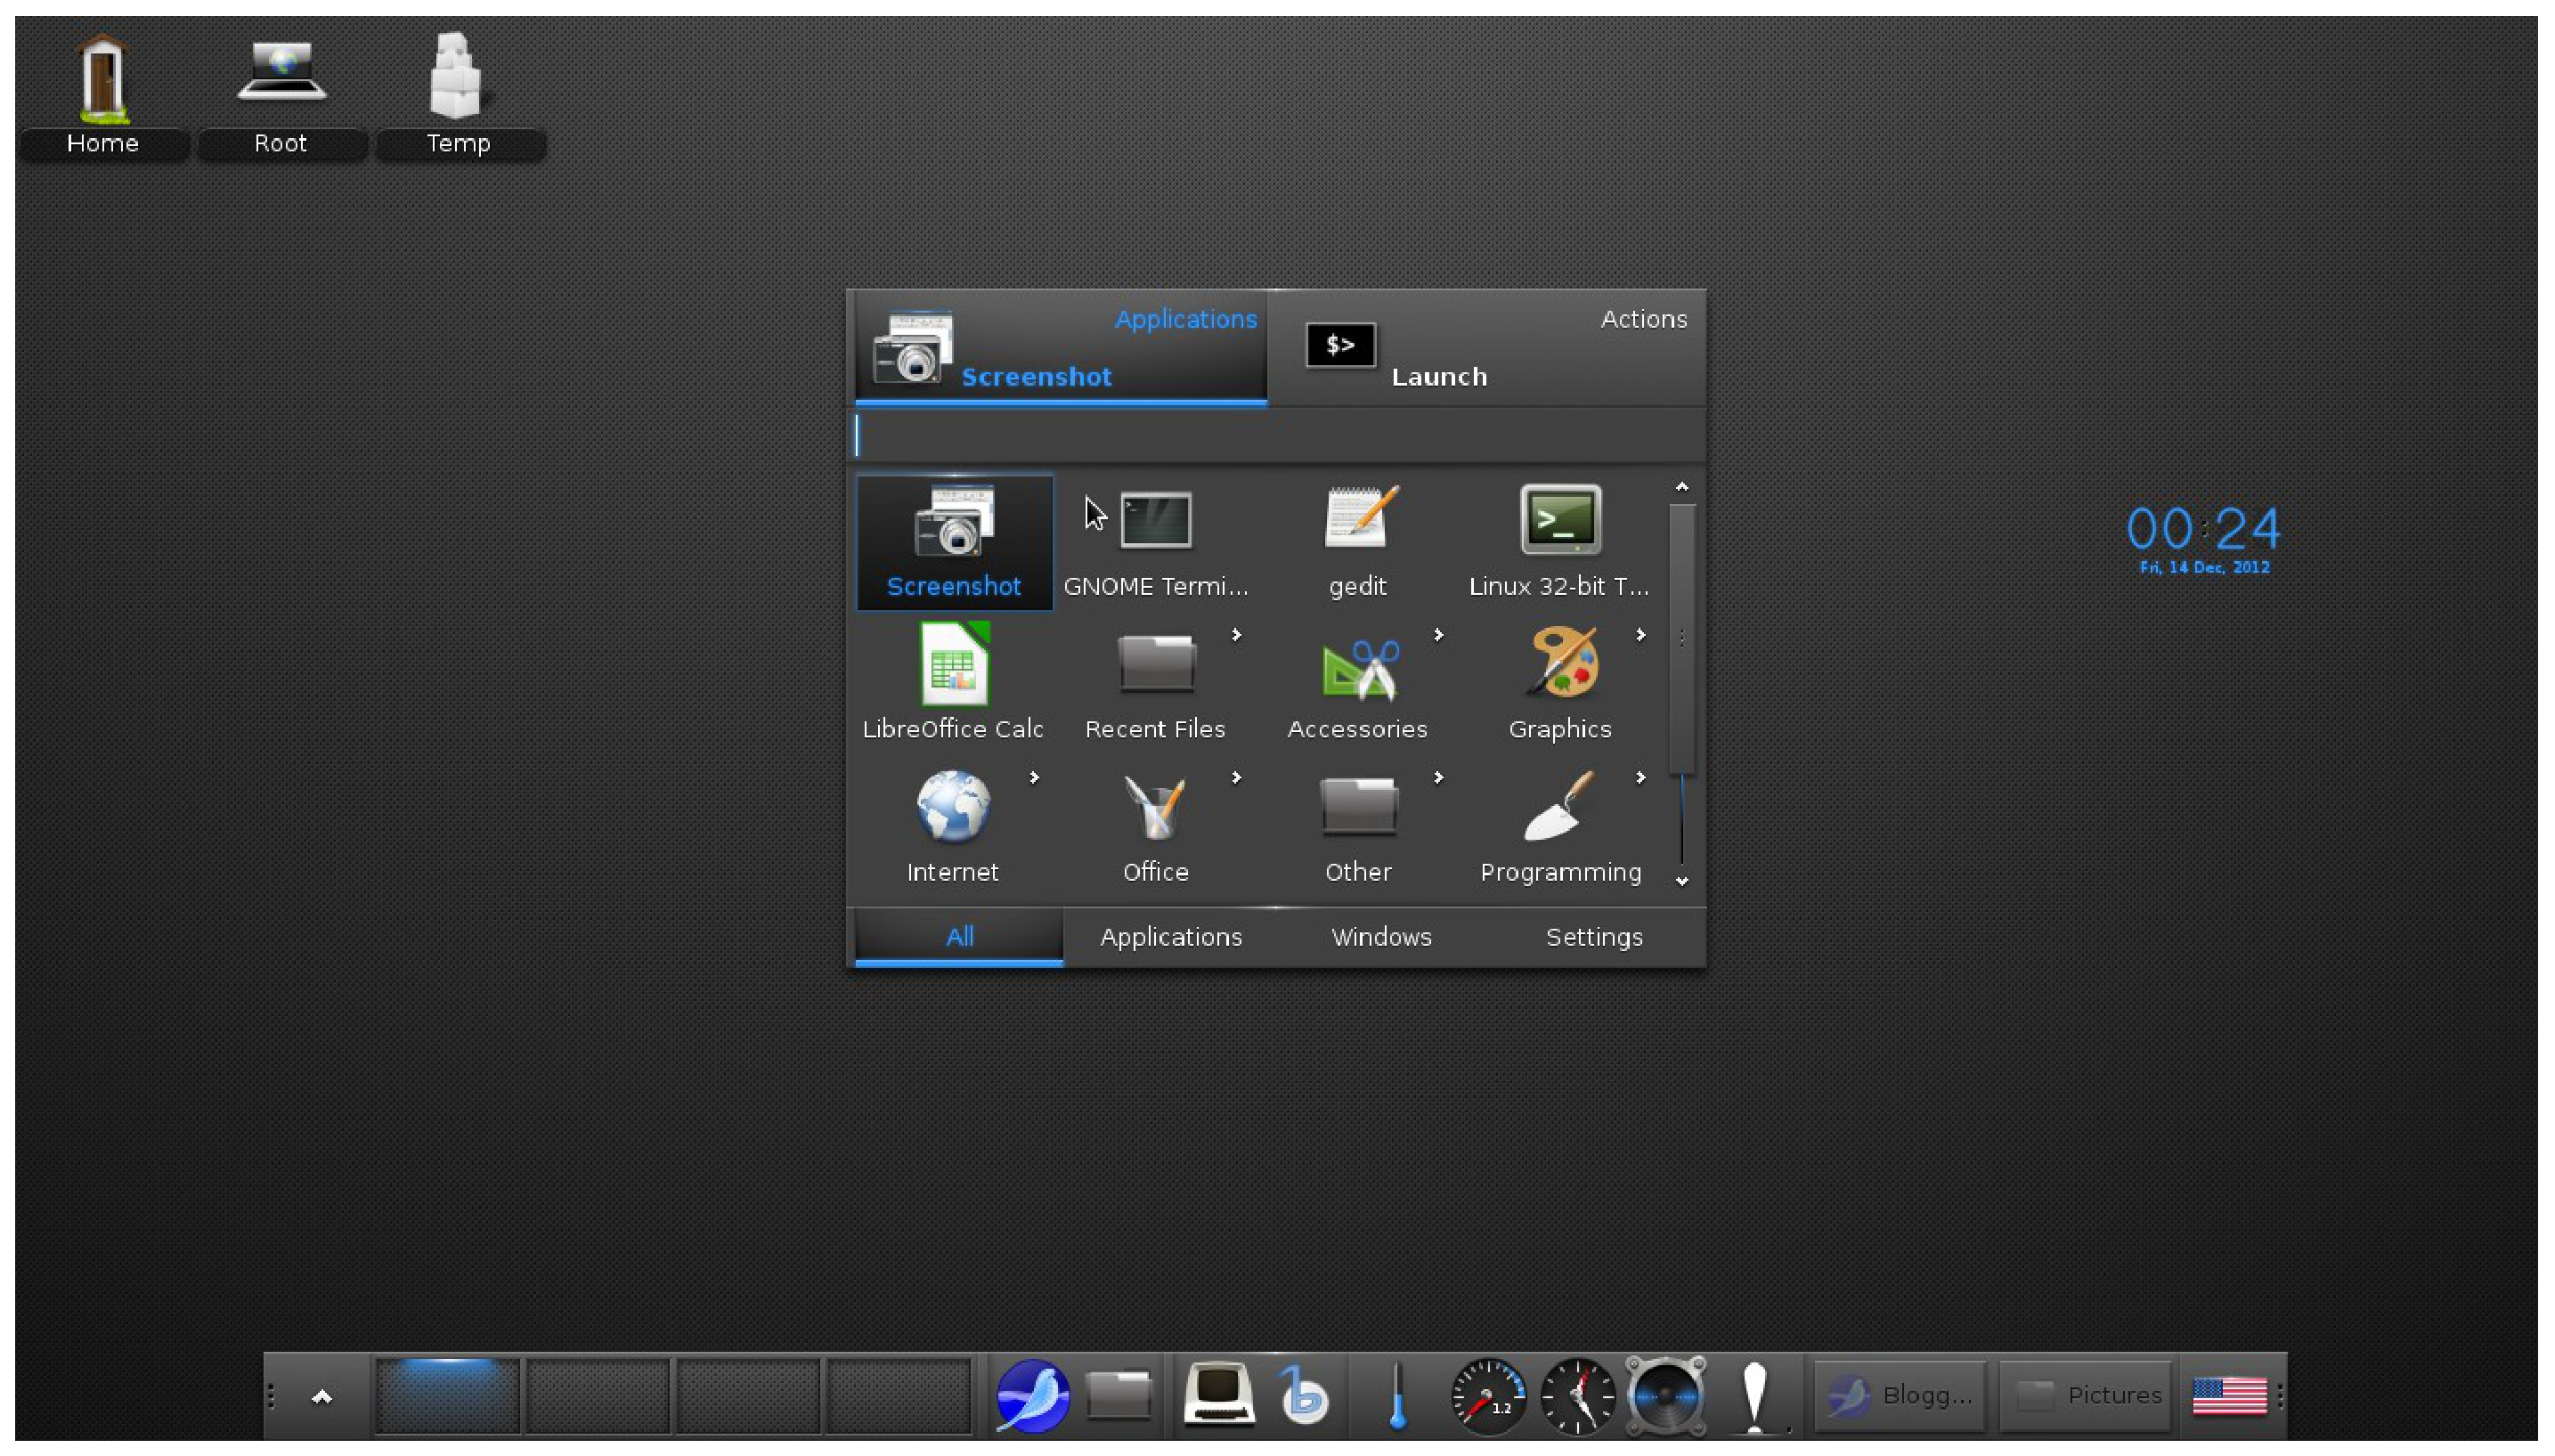
\includegraphics[width=\linewidth]{img/RunEverything.eps}
    \end{frame}

    \begin{frame}{The man with the golden panel}
        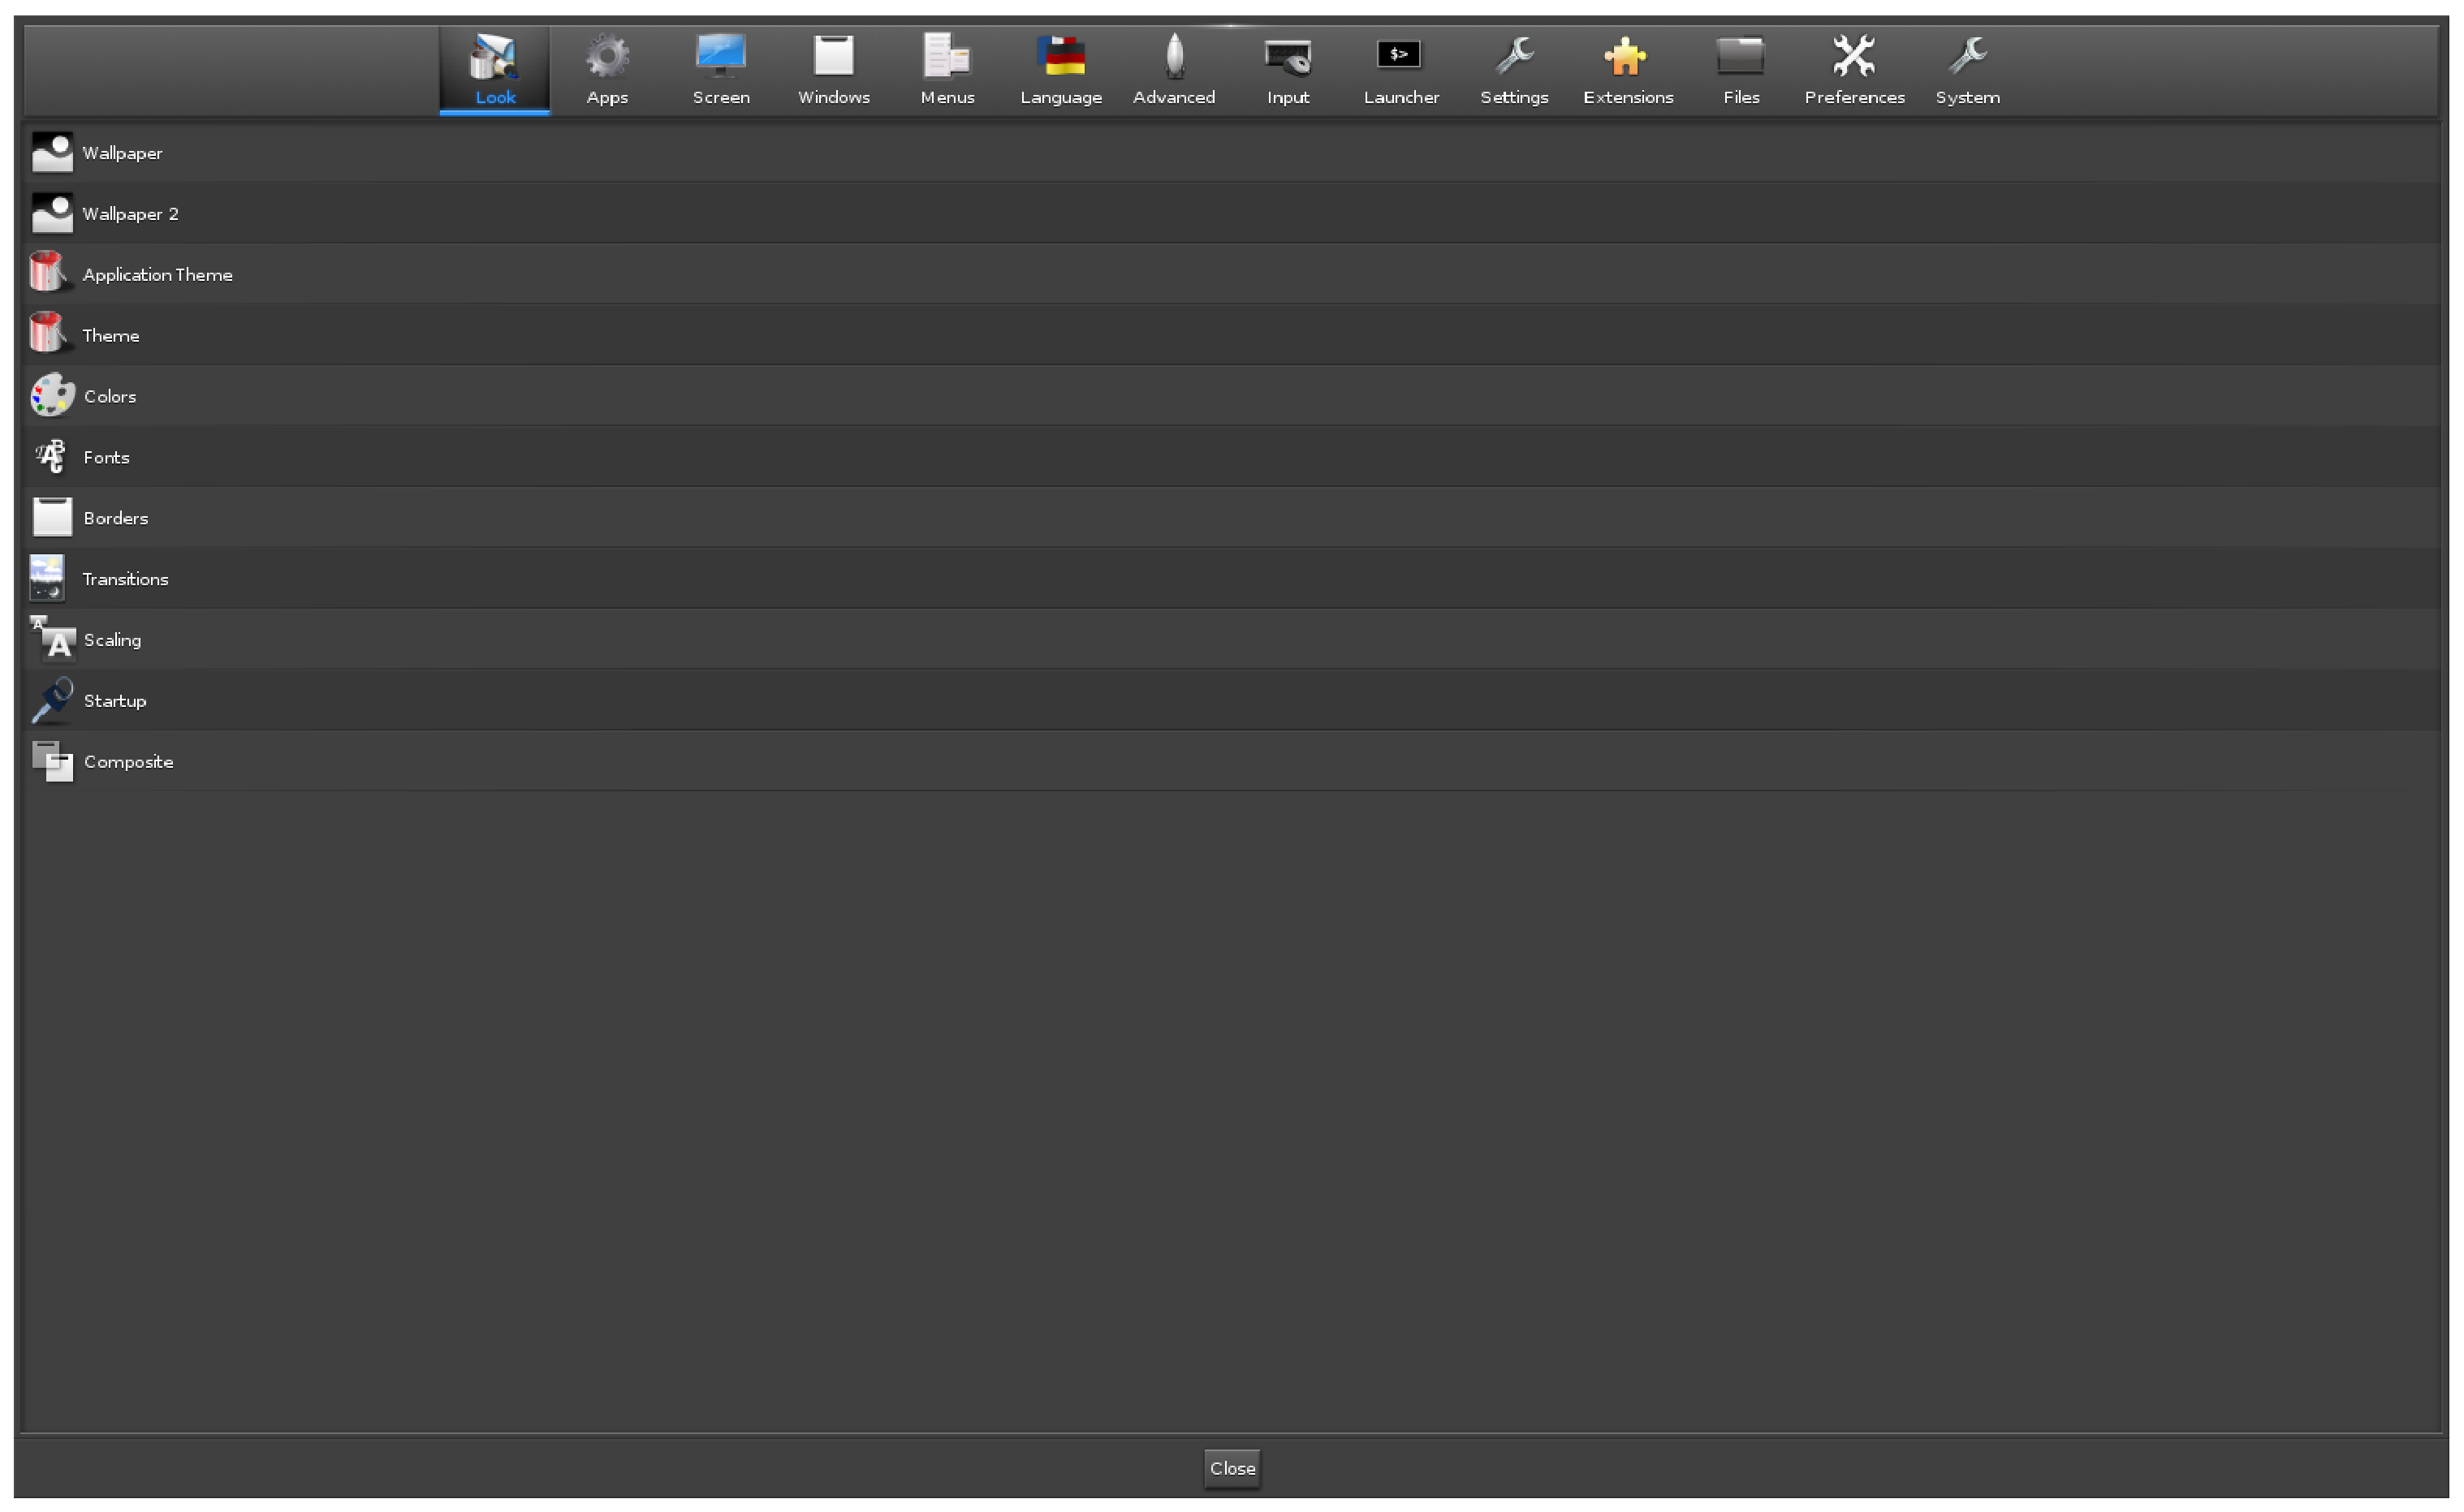
\includegraphics[width=\linewidth]{img/Settings-Panel.eps}
    \end{frame}

    \begin{frame}
        \center\huge But there is more\ldots
    \end{frame}

    \begin{frame}{Beyond the desktop}
        \begin{block}{Embedded Systems}
            \begin{itemize}
                \item Infinity I-Kitchen
                \item SetTopBoxes by Free.fr
                \item Special laptops and services by ordissimo
                \item Mobile/TV/Tablet/IVI with Tizen
            \end{itemize}
        \end{block}
    \end{frame}

    \begin{frame}{Electrolux}{Infinity I-Kitchen}
        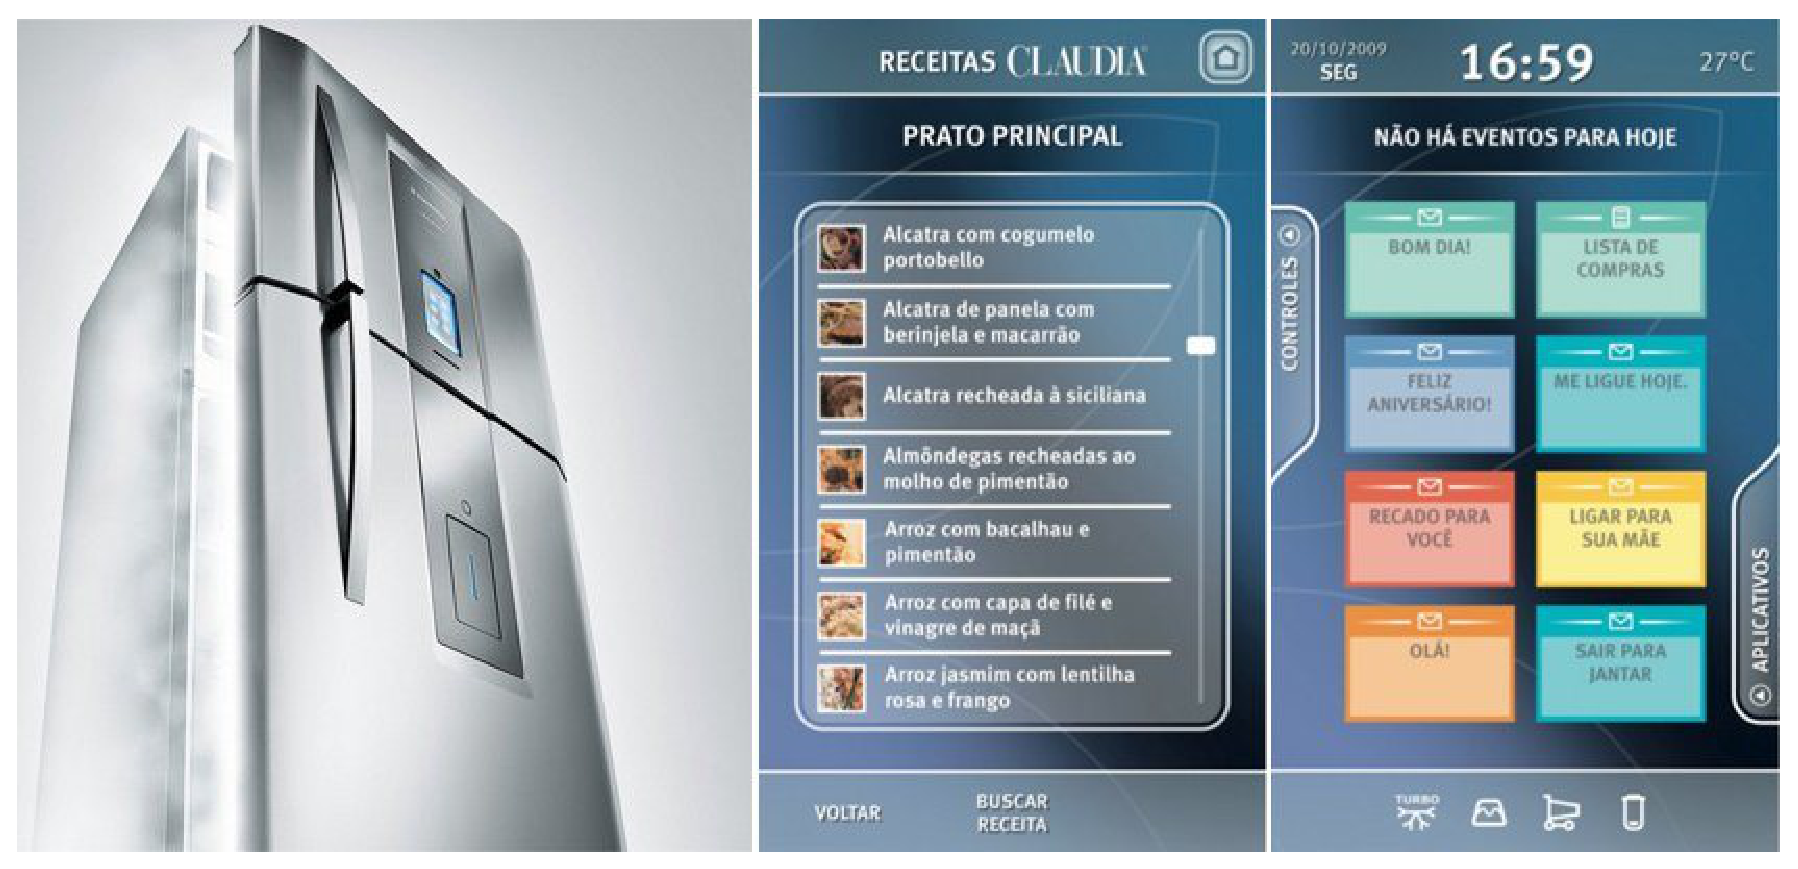
\includegraphics[width=\linewidth]{img/frigorifico-infinity-i-kitchen.eps}
    \end{frame}

    \begin{frame}{Ordissimo}{Laptop interface}
        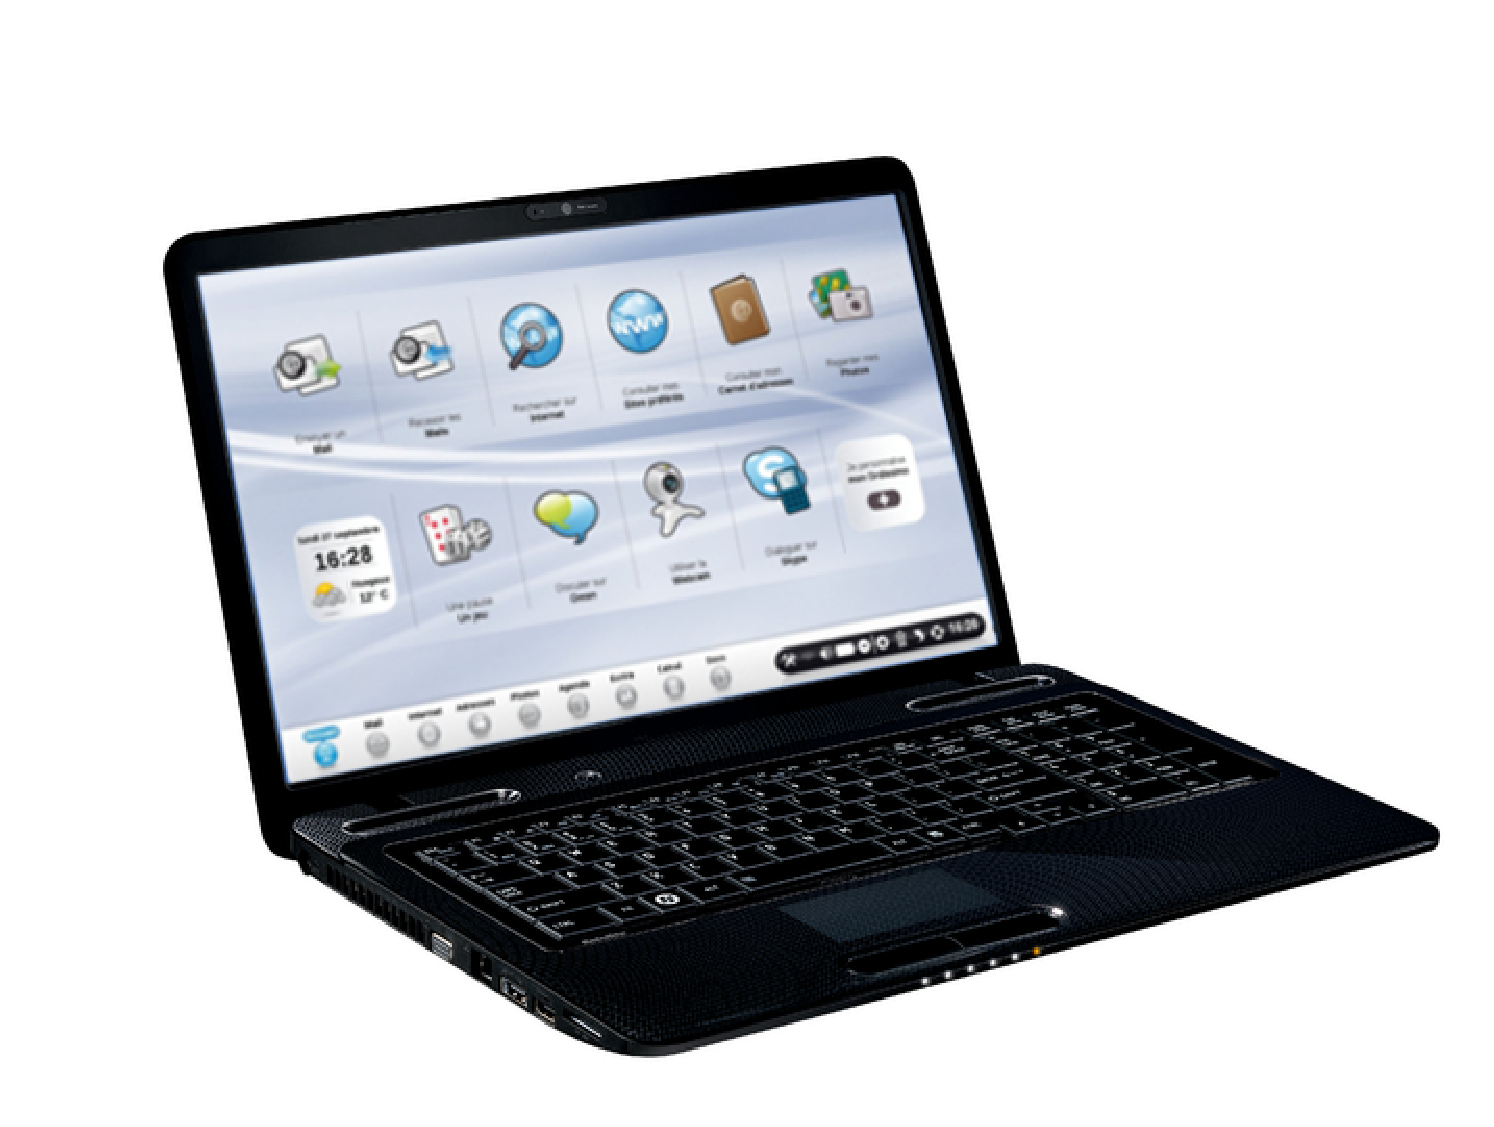
\includegraphics[width=\linewidth]{img/ordissimo.eps}
    \end{frame}

    \begin{frame}{Samsung}{Tizen}
        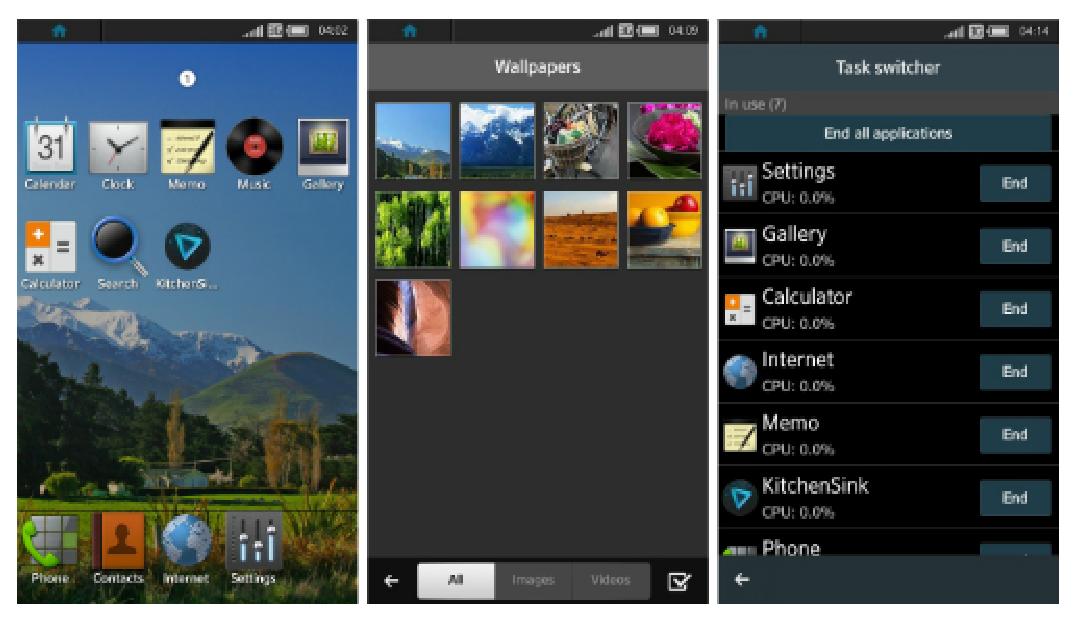
\includegraphics[width=\linewidth]{img/Tizen-UI1.eps}
    \end{frame}

    \begin{frame}
        \center\huge The Philosophy\ldots \\
        or \\
        How i learned to stop worrying and LOVE\\
        the Enlightenment.
    \end{frame}

    \begin{frame}
        \center CHOICE IS GOOD
    \end{frame}

    \begin{frame}
        \center Vanilla vs. Strawberry vs. Chocolate
    \end{frame}

    \begin{frame}
        \center EFFICIENCY MATTERS
    \end{frame}

    \begin{frame}
        \center NOT everyone drives an F1
    \end{frame}

    \begin{frame}
        \center EYECANDY MATTERS
    \end{frame}

    \begin{frame}
        \center PORTING MATTERS
    \end{frame}

    \begin{frame}
        \center The world is NOT english
    \end{frame}

    \begin{frame}
        \center OPEN IS BEST
    \end{frame}
        
    \begin{frame}
        \center We have a sense of humor
    \end{frame}

    \begin{frame}{How can i get it?}
        \begin{itemize}
            \item {\bf e17} is already in the core distribution repos and can be
                  chosen as an option from the installation media
                  (the full dvd).
            \item {\bf enlightenment} The current upstream version ({\bf 0.19.12} as of
                  this talk can be installed from the repository
                  {\bf X11:Enlightenment:Factory} found in the url below
                  (choose the link for your running distro version)
                  \url{http://en.opensuse.org/Portal:Enlightenment}
        \end{itemize}
    \end{frame}

    \begin{frame}{I want in!}{Being part of the effort}
        \center\huge Setting up a development environment for Enlightenment
    \end{frame}

    \begin{frame}{Build Essentials}
        \begin{block}{Git to fetch the code}
            \# zypper install git-core
        \end{block}
        \begin{block}{Tracing tool \& test suite}
            \# zypper install check valgrind
        \end{block}
        \begin{block}{C/C++ Development Pattern}
            \# zypper install -t pattern devel\_C\_C++
        \end{block}
    \end{frame}

    \begin{frame}{Contact}
        \begin{block}{IRC}
            irc.freenode.net    \#e \\
            irc.freenode.net    \#e.el \\
            irc.freenode.net    \#opensuse-e \\
            irc.freenode.net    \#opensuse-el
        \end{block}
    \end{frame}

    \begin{frame}{Bug Reporting / Bug Hunting}
        \begin{block}{Phabricator}
            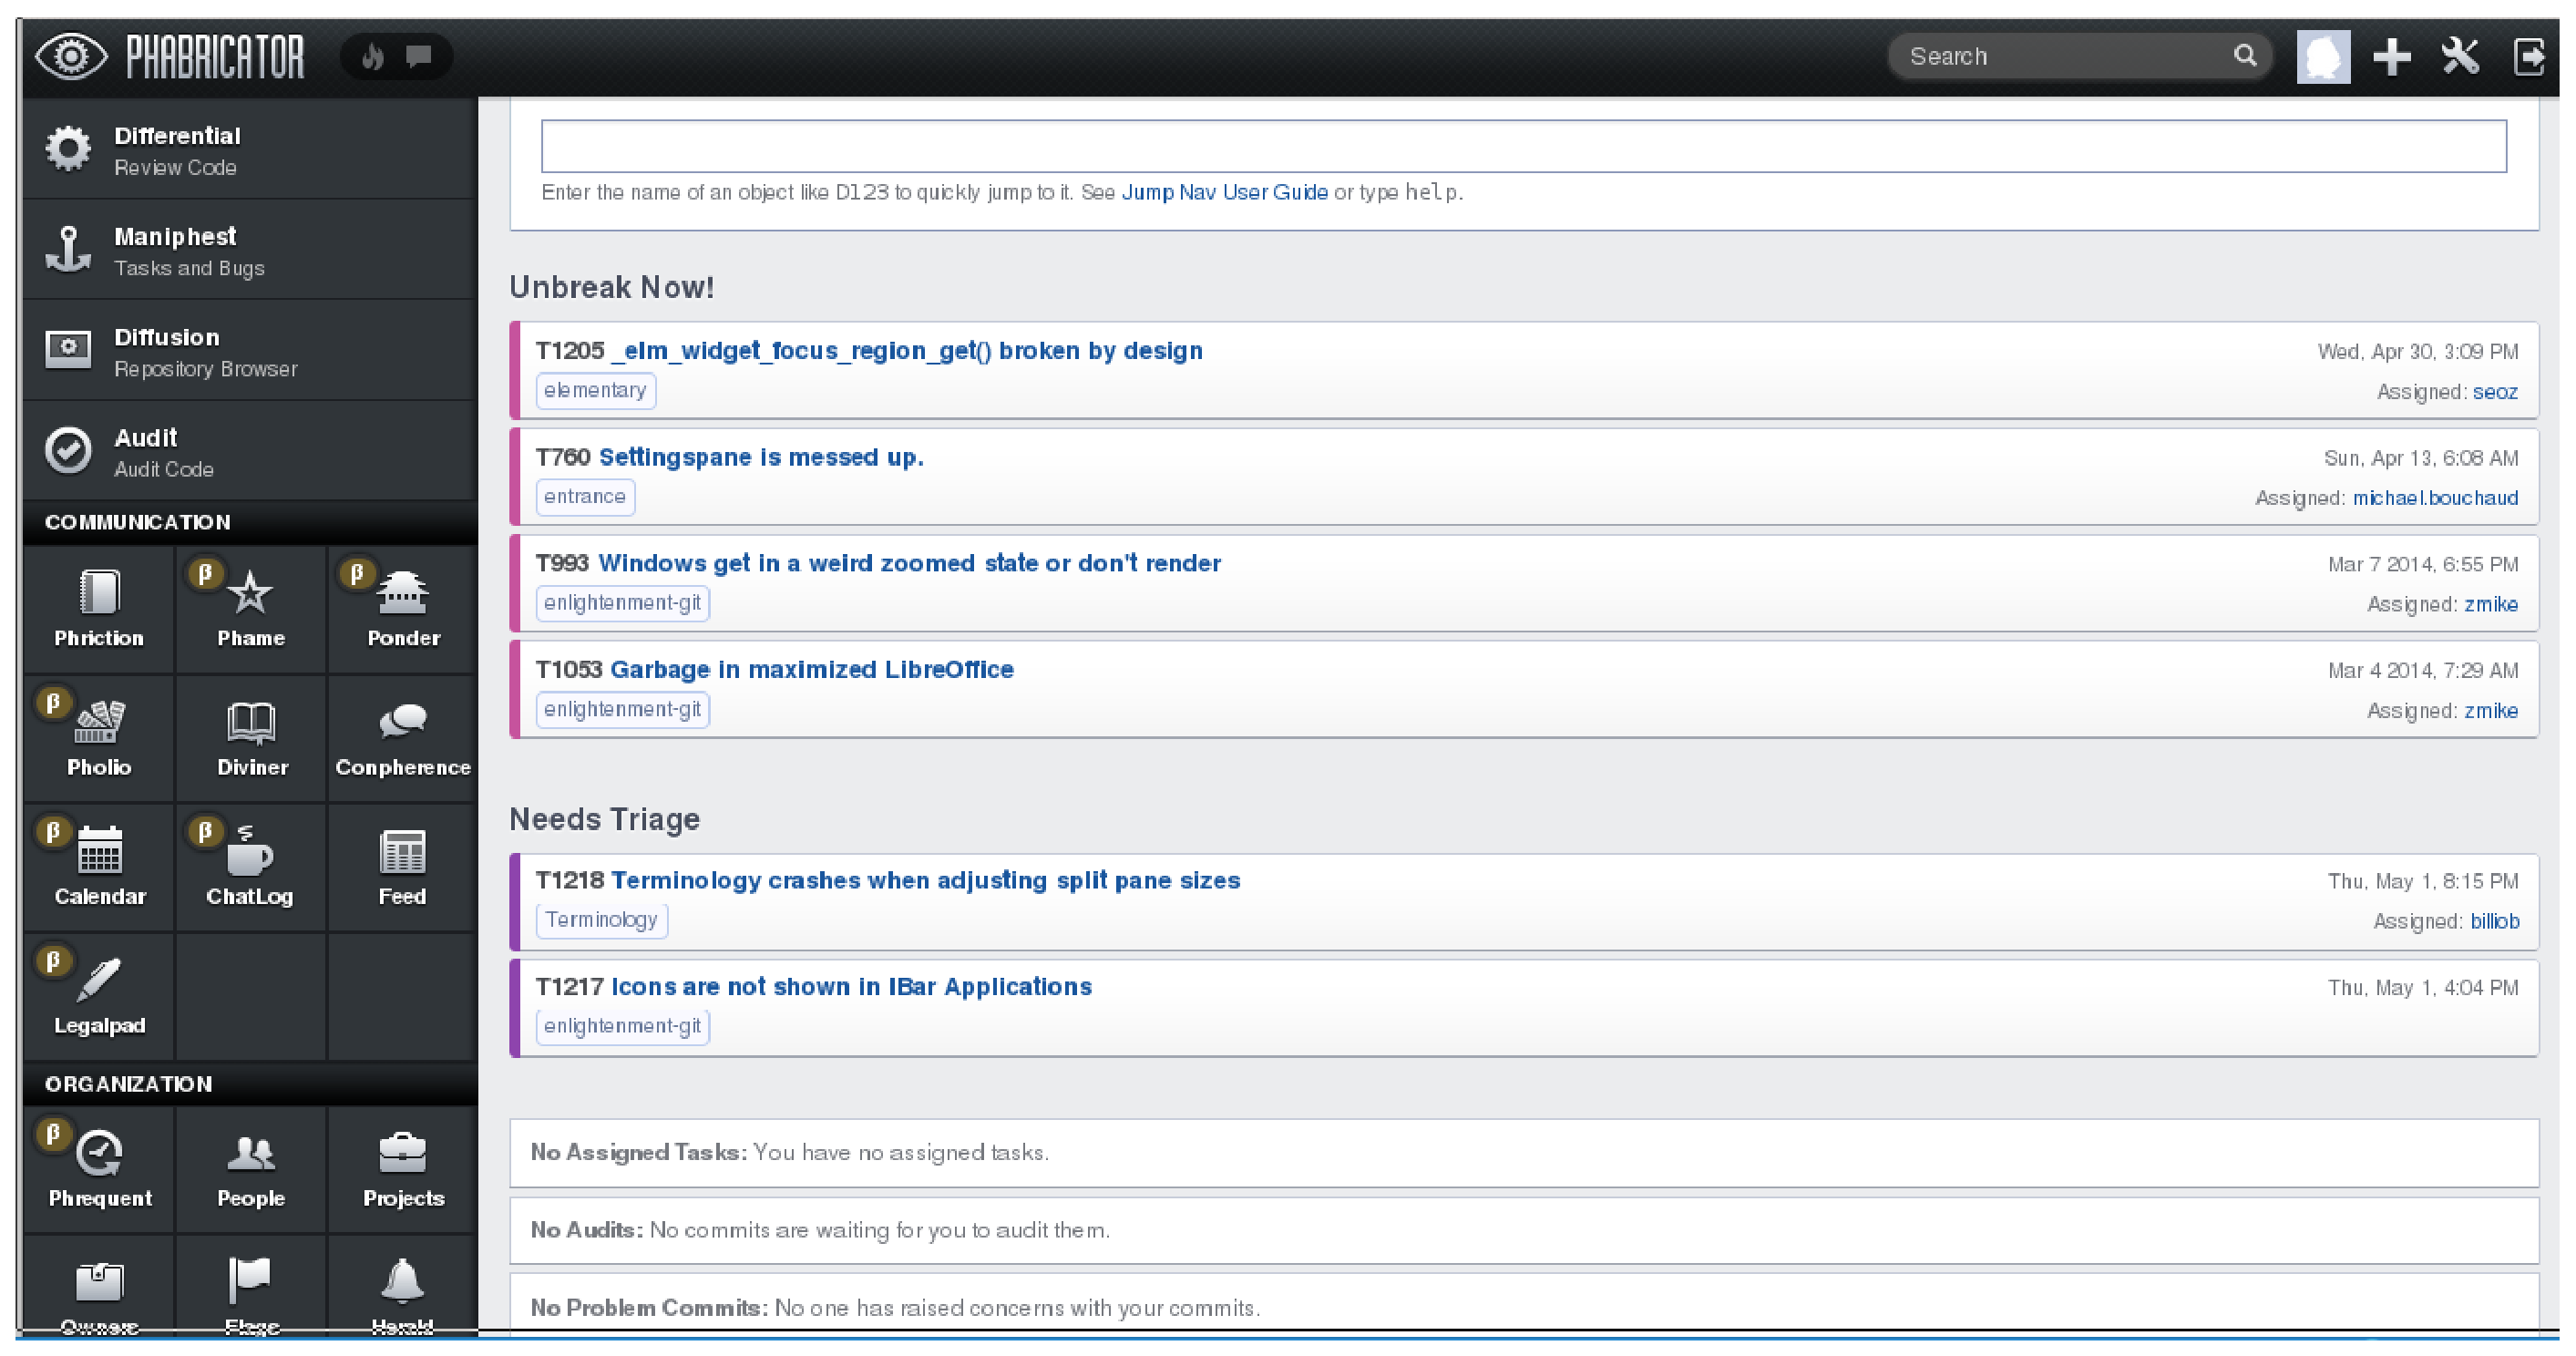
\includegraphics[width=\linewidth]{img/phab.eps}
        \end{block}
    \end{frame}

    \begin{frame}{The Greek (localization) effort}
        Wiki portal fully translated in Greek \\
        Enlightenment \& EFL Translations are currently @ 95\%
    \end{frame}

    \begin{frame}{Q \& A}{Thank you for your attention!}
        \center Alex-P. Natsios\\
        \center\url{drakevr@2f30.org}\\
        \center\url{http://drakevr.gr}\\
        \center\url{http://www.linkedin.com/in/drakevr}\\
        \center\url{http://www.github.com/drakevr}\\
        \center\url{http://www.facebook.com/drakevr}\\
        \center\url{http://www.twitter.com/drakevr}
    \end{frame}

\end{document}
